\documentclass[a4paper,14pt]{extreport} % формат документа

\usepackage{amsmath}
\usepackage{cmap} % поиск в ПДФ
\usepackage[T2A]{fontenc} % кодировка
\usepackage[utf8]{inputenc} % кодировка исходного текста
\usepackage[english,russian]{babel} % локализация и переносы
\usepackage[left = 2cm, right = 1cm, top = 2cm, bottom = 2 cm]{geometry} % поля
\usepackage{listings}
\usepackage{graphicx} % для вставки рисунков
\usepackage{amsmath}
\usepackage{float}
\usepackage{multirow}
\graphicspath{{img/}}
\DeclareGraphicsExtensions{.pdf,.png,.jpg}
\newcommand{\anonsection}[1]{\section*{#1}\addcontentsline{toc}{section}{#1}}

\lstset{ %
	language=Lisp,                % Язык программирования 
	numbers=left,                   % С какой стороны нумеровать          
	frame=single,                    % Добавить рамку
}

\begin{document}
\begin{titlepage}

    \begin{table}[H]
        \centering
        \footnotesize
        \begin{tabular}{cc}
            \multirow{8}{*}{
\includegraphics[scale=0.35]{bmstu.jpg}}
            & \\
            & \\
            & \textbf{Министерство науки и высшего образования Российской Федерации} \\
            & \textbf{Федеральное государственное бюджетное образовательное учреждение} \\
            & \textbf{высшего образования} \\
            & \textbf{<<Московский государственный технический} \\
            & \textbf{университет имени Н.Э. Баумана>>} \\
            & \textbf{(МГТУ им. Н.Э. Баумана)} \\
        \end{tabular}
    \end{table}

    \vspace{-2.5cm}

    \begin{flushleft}
        \rule[-1cm]{\textwidth}{3pt}
        \rule{\textwidth}{1pt}
    \end{flushleft}

    \begin{flushleft}
        \small
        ФАКУЛЬТЕТ
        \underline{<<Информатика и системы управления>>\ \ \ \ \ \ \ 
        \ \ \ \ \ \ \ \ \ \ \ \ \ \ \ \ \ \ \ \ \ \ \ \ \ \ \ \ \ \ \ 
    \ \ \ \ \ \ \ \ \ \ \ \ \ \ \ } \\
        КАФЕДРА
        \underline{<<Программное обеспечение ЭВМ и
        информационные технологии>>
        \ \ \ \ \ \ \ \ \ \ \ \ \ \ \ \ \ \ \ \ }
    \end{flushleft}

    \vspace{2cm}

    \begin{center}
        \textbf{Лабораторная работа № 3} \\
        \vspace{0.5cm}
    \end{center}

    \vspace{4cm}

    \begin{flushleft}
        \begin{tabular}{ll}
            \textbf{Дисциплина} & Экономика программной инженерии.  \\
            \textbf{Тема} & Оптимизация параметров проекта. \\
            & Выравнивание загрузки ресурсов. Учет периодических задач. \\
            & Минимизация критического пути \\
            \\
            \textbf{Студент} & Сусликов Д.В. \\
            \textbf{Группа} & ИУ7-85Б \\
            \textbf{Оценка (баллы)} & \\
            \textbf{Преподаватель} & Барышникова М.Ю., Силантьева А.В.   \\
        \end{tabular}
    \end{flushleft}

    \vspace{4cm}

   \begin{center}
        Москва, 2022 г.
    \end{center}

\end{titlepage}

\begin{enumerate}

\item \textbf{Основное задание}

Содержание проекта: Команда разработчиков из 16 человек занимается созданием карты города на основе собственного модуля отображения. Проект должен быть завершен в течение 6 месяцев. Бюджет проекта: 50 000 рублей.

\item \textbf{Выравнивание загрузки ресурсов в проекте}

Причины перегрузки ресурсов, получившейся как результат выполнения лабораторной работы №2: использование одного ресурса одновременно в двух задачах. Ниже пример.

\begin{figure}[H]
  \centering
  \caption{Перегрузка. }
  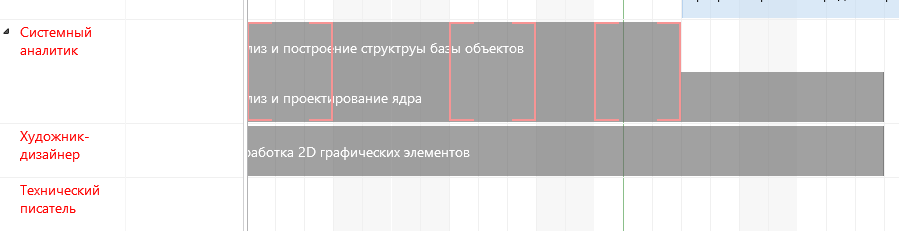
\includegraphics[scale=0.7]{1}
\end{figure}

В соответствии с первым заданием в проекте была произведена ликвидация перегрузки ресурсов при помощи автоматических параметров выравнивания. Автоматическое выравнивание -- задачи, в которых задействованы перегруженные ресурсы, смещаются, при этом первыми на выполнение ставятся критические задачи необходимые для успешного завершения проекта.

\begin{figure}[H]
  \centering
  \caption{Ликвидация перегрузки. }
  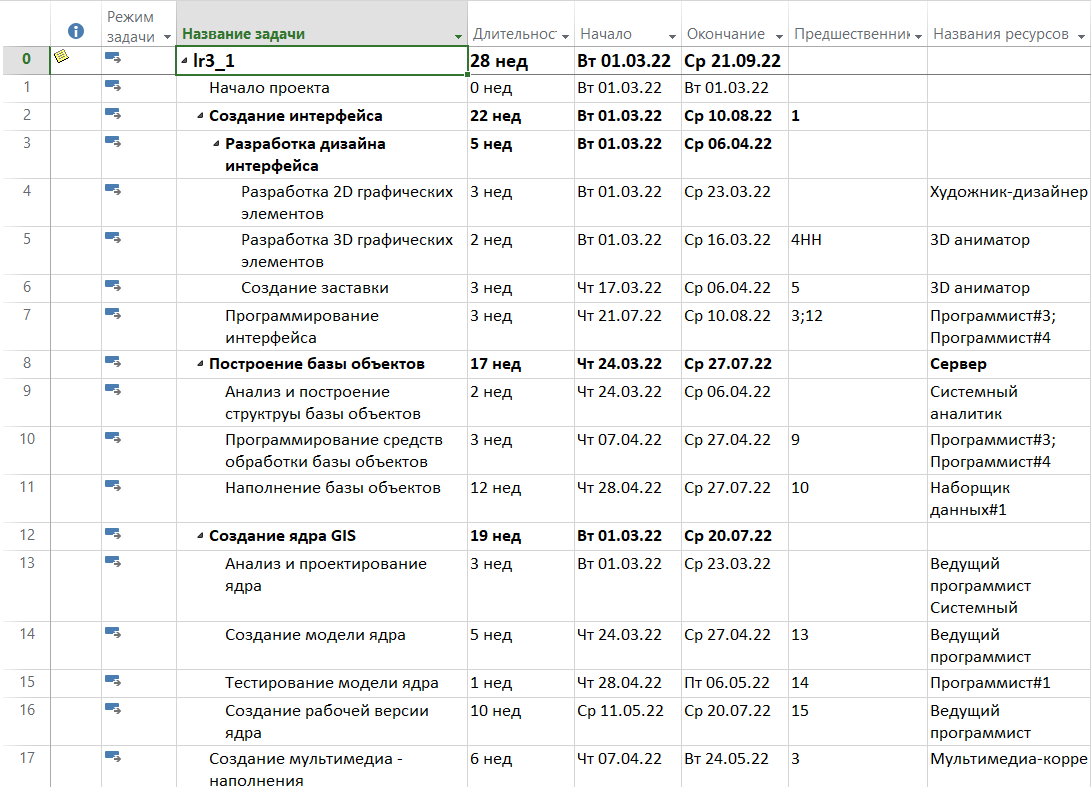
\includegraphics[scale=0.7]{2}
\end{figure}

\begin{figure}[H]
	\centering
	\caption{Ликвидация перегрузки. }
	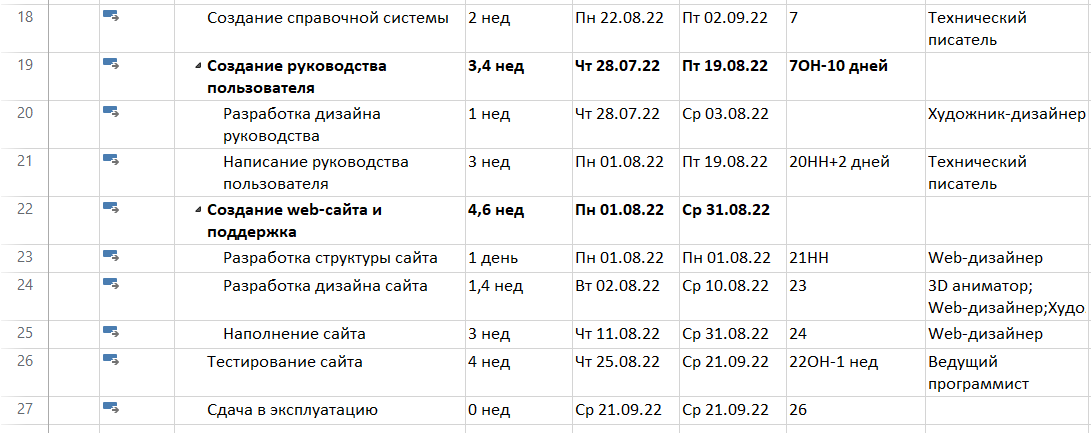
\includegraphics[scale=0.7]{22}
\end{figure}
\item \textbf{Учет периодических задач в плане проекта}

Добавляем задачу совещание с периодичностью в 1 неделю по средам длительностью чвс.

\begin{figure}[H]
  \centering
  \caption{Совещание. }
  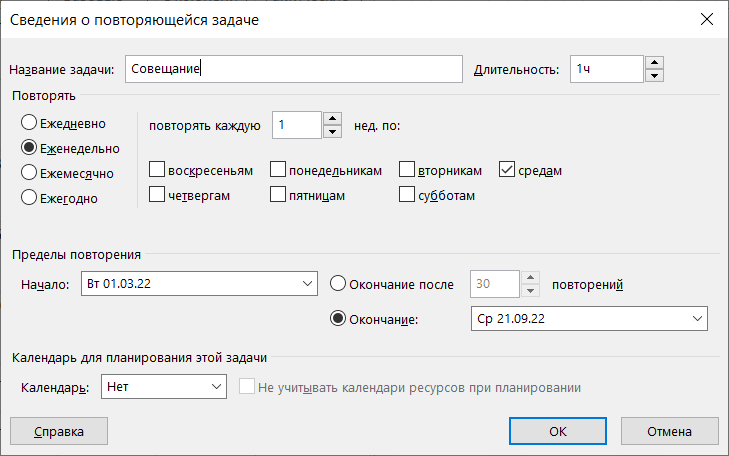
\includegraphics[scale=0.8]{3}
\end{figure}

Добавляем сотрудников.

\begin{figure}[H]
  \centering
  \caption{Сотрудники на совещании. }
  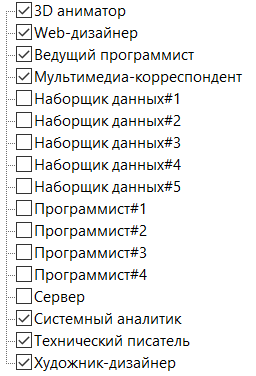
\includegraphics[scale=0.8]{4}
\end{figure}

 Устраняем с помощью автоматического выравнивания по часам.

\begin{figure}[H]
  \centering
  \caption{Автоматическое выравнивание по часам. }
  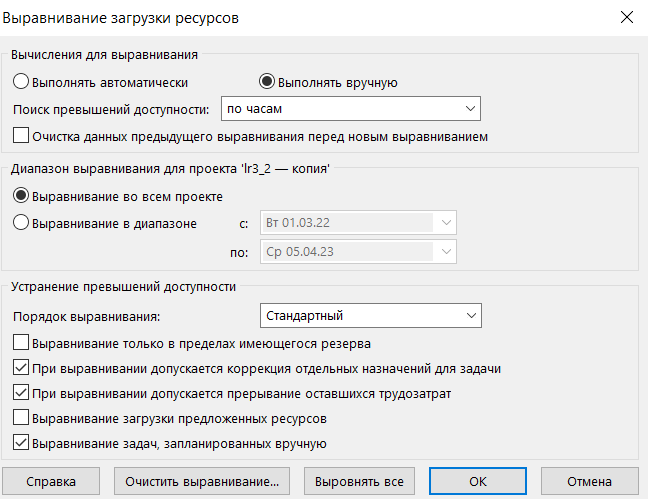
\includegraphics[scale=0.8]{6}
\end{figure}

После выравниваний затраты вышли из бюджета и сильно сдвинулась дата окончания проекта:

\begin{figure}[H]
  \centering
  \caption{Полученные неудовлетворительные результаты. }
  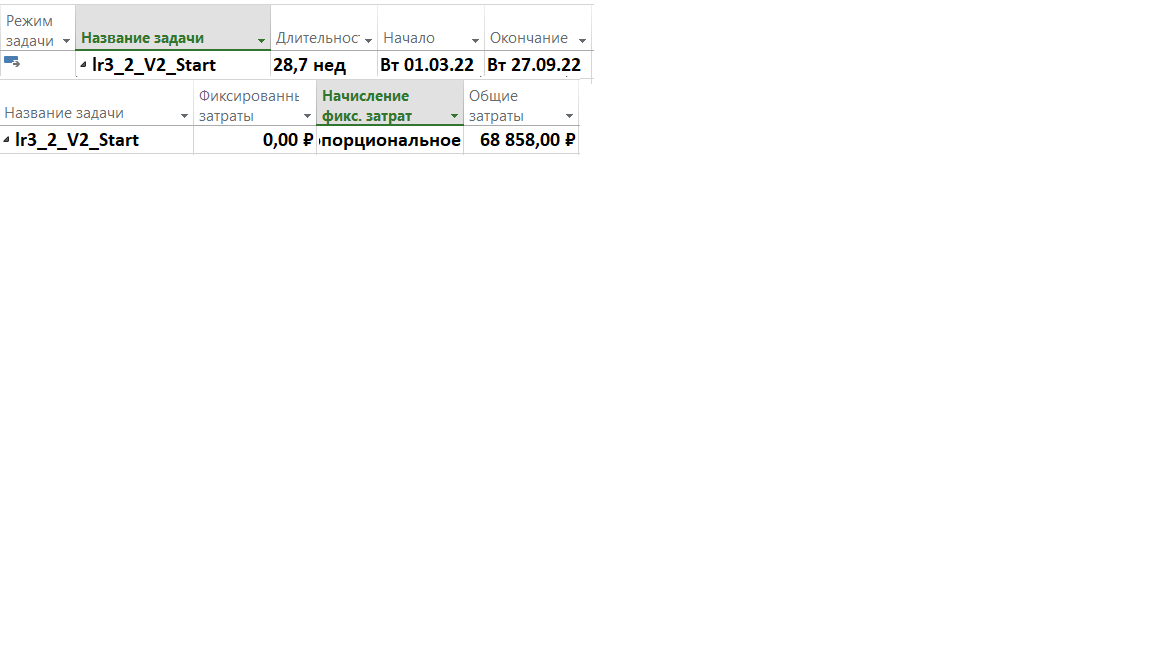
\includegraphics[scale=0.9]{7}
\end{figure}

Настроим сведения о затратах каждого сотрудника, который участвует в совещании, так как не будем платить затрату на использование в совещании.

\begin{figure}[H]
  \centering
  \caption{Сведения о затратах каждого сотрудника. }
  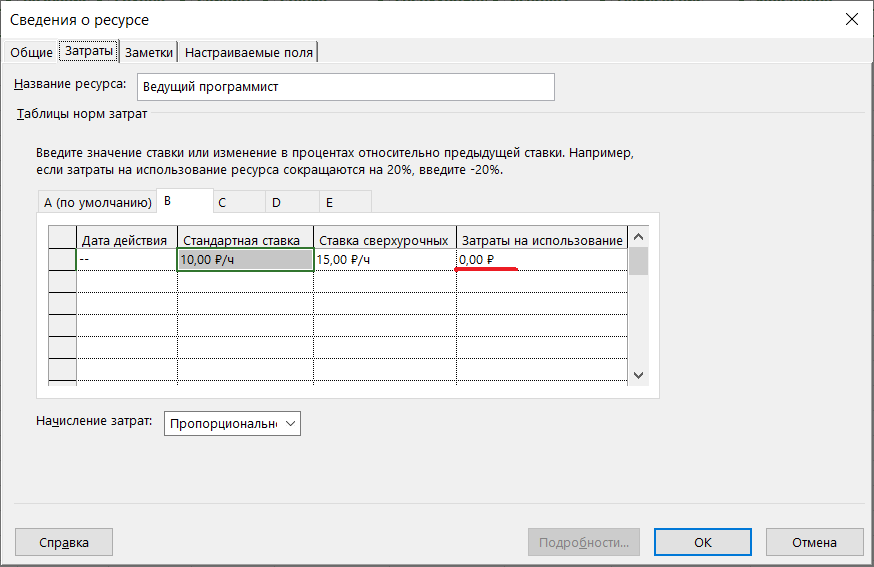
\includegraphics[scale=0.9]{9}
\end{figure}

Назначим тип затрат для сотрудников на совещании:

\begin{figure}[H]
  \centering
  \caption{Назначение типа затрат для сотрудников. }
  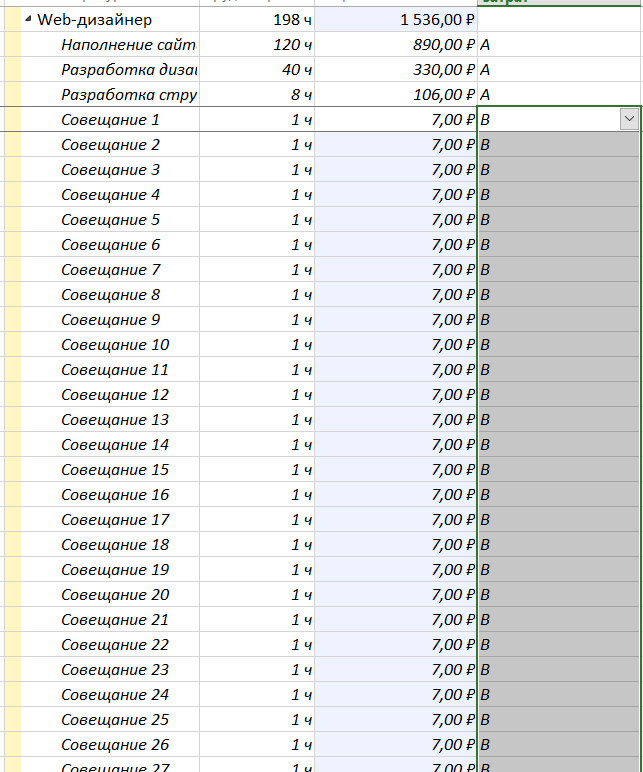
\includegraphics[scale=0.9]{10}
\end{figure}

Тогда получаем:

\begin{figure}[H]
  \centering
  \caption{После изменений. }
  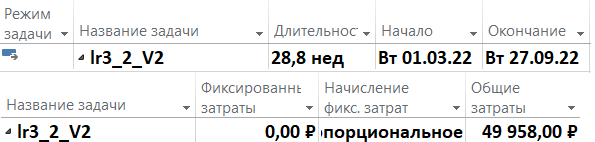
\includegraphics[scale=0.9]{11}
\end{figure}

Бюджет соответсвтует требуемому условию в 50000, однако срок окончания работы -- нет, поэтому следует провести отпимизацию по времени.

Для этого назначим на все задачи, в которых участвуют не все программисты, всех свободных. Так получилось добавить рабочие ресуры в задачи 7, 10, 14, 15, 16, 26

\begin{figure}[H]
	\centering
	\caption{Назначение программистов. }
	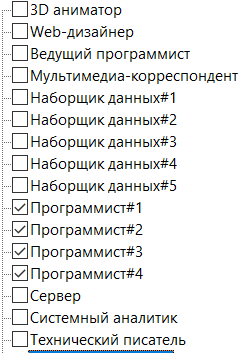
\includegraphics[scale=0.9]{8}
\end{figure}

Тогда получаем удовлетворительные результаты:

\begin{figure}[H]
	\centering
	\caption{После оптимизации. }
	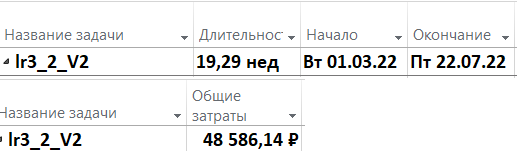
\includegraphics[scale=0.9]{112}
\end{figure}

\item \textbf{Оптимизация критического пути}

Для оптимизации мы добавили в задачи связанные с программированием дополнительных программистов. И также сократили сроки проведения совещаний.

Оптимизированный критический путь.

\begin{figure}[H]
  \centering
  \caption{Критический путь. }
  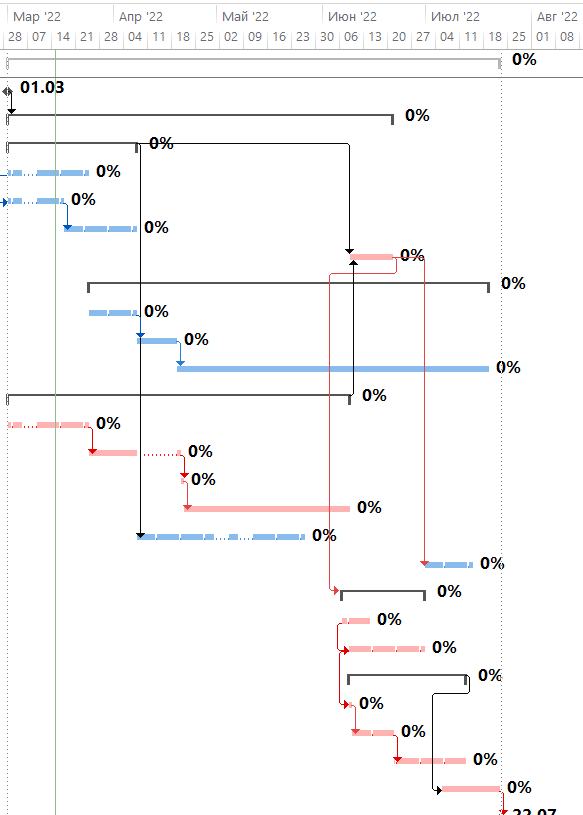
\includegraphics[scale=0.9]{12}
\end{figure}

Далее приведем статистику затрат и трудозатрат, для графического представления воспользуемся Google Docs.

\begin{figure}[H]
  \centering
  \caption{Таблица. }
  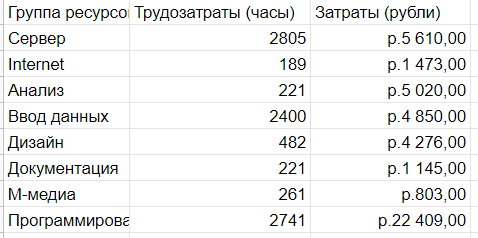
\includegraphics[scale=1]{table}
\end{figure}

\begin{figure}[H]
  \centering
  \caption{Информация о затратах по структурным группам ресурсов. }
  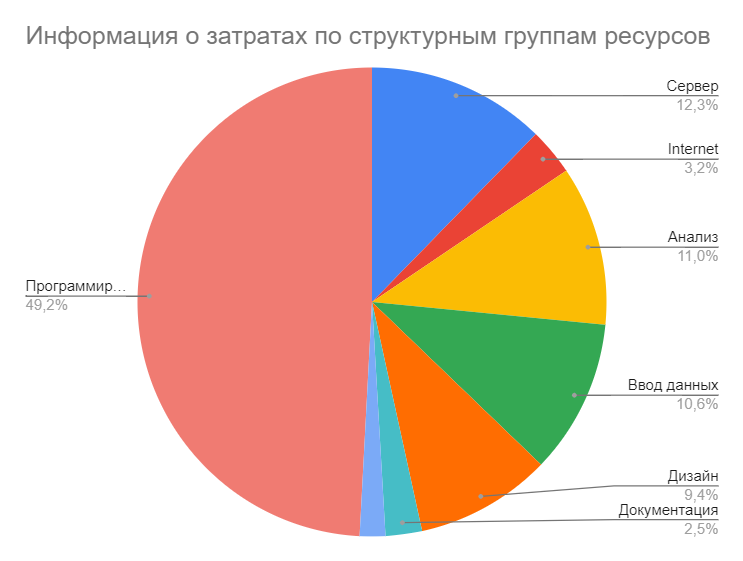
\includegraphics[scale=1]{d1}
\end{figure}

\begin{figure}[H]
  \centering
  \caption{Информация о трудозатратах по структурным группам ресурсов. }
  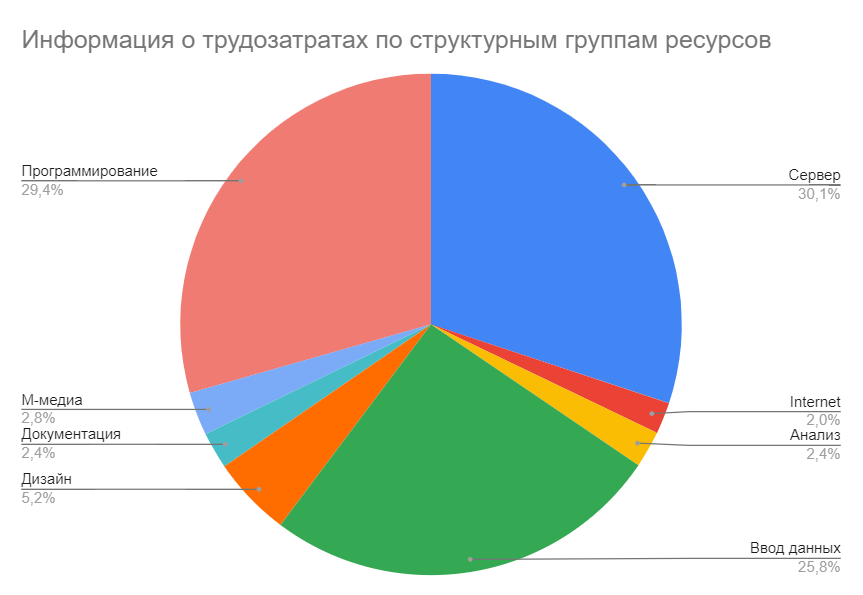
\includegraphics[scale=1]{d2}
\end{figure}

Как видим, на программистов приходится большая часть и затрат 49.2\%, и трудозатрат 29.4\%.

Cервер остается вторым по размеру затрат -- 12.3\%.

Статистика трудозатрат и затрат не претерпела сильных изменений.

Далее сохраним базовый план.

\begin{figure}[H]
  \centering
  \caption{Базовый план. }
  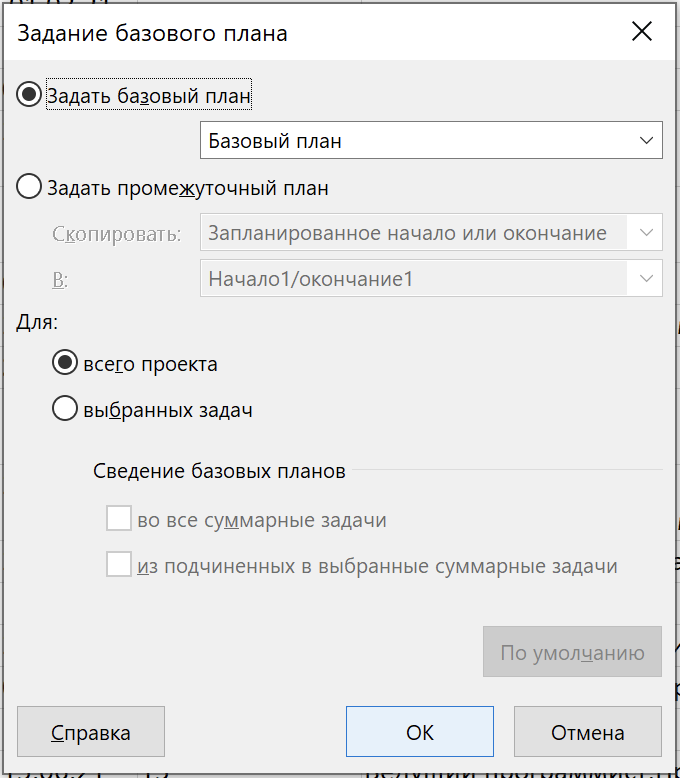
\includegraphics[scale=0.75]{13}
\end{figure}


\item \textbf{Вывод}

В результате выполнения лабораторной работы, в проекте были учтены еженедельные совещания по средам.

Также была произведена разгрузка использованных ресурсов и оптимизация финансовых и временных затрат. В итоге, проект укладывается как в рамки бюджета: затраты -- 48.586,14 рублей, так и во временные рамки -- срок окончания 22 июля. 

Ресурсы в проекте не перегружены.

\end{enumerate}

\end{document}